\documentclass[11pt,a4paper]{article}

\usepackage[margin=1in]{geometry}
\usepackage{setspace}
\usepackage{titlesec}
\usepackage{enumitem}
\usepackage{hyperref}
\usepackage{tikz}
\usetikzlibrary{positioning,shapes,arrows.meta}

\setlist[itemize]{topsep=4pt,itemsep=2pt,leftmargin=1.2cm}
\setlist[enumerate]{topsep=4pt,itemsep=2pt,leftmargin=1.2cm}
\setstretch{1.15}
\titleformat{\section}{\normalfont\Large\bfseries}{\thesection}{0.5em}{}
\titleformat{\subsection}{\normalfont\large\bfseries}{\thesubsection}{0.5em}{}

\title{Hostel Management System \\ \large Software Requirements Specification}
\author{Prepared for: Project Presentation}
\date{\today}

\begin{document}
\maketitle

\section{Introduction}
\subsection{Purpose}
This document describes the Software Requirements Specification (SRS) for the Hostel Management System that digitizes hostel admissions, room allocation, staff tracking, and student services. It aligns stakeholders---administrators, staff supervisors, and students---on the expected functionality, constraints, and quality attributes before development and deployment.

\subsection{Background \& Motivation}
Manual record keeping leads to inconsistent data, limited transparency, and difficult auditing. The proposed system provides a centralized web portal (React client) backed by a Node.js/Express API and MongoDB database. It enforces controlled access through role-based authentication so that a single administrator can manipulate records while students have read-only visibility of their data.

\subsection{Definitions \& References}
\begin{itemize}
  \item JWT --- JSON Web Token used for stateless authentication.
  \item CRUD --- Create, Read, Update, Delete.
  \item MERN stack --- MongoDB, Express.js, React.js, Node.js.
  \item Reference: Official documentation of React (\url{https://react.dev}), Express (\url{https://expressjs.com}), and MongoDB (\url{https://www.mongodb.com}).
\end{itemize}

\section{Objectives and Scope}
\subsection{Objectives}
\begin{enumerate}
  \item Provide a secure portal where the designated hostel administrator manages rooms, staff, and student records.
  \item Offer students a personalized dashboard showing their room assignment, leave status, and profile with read-only access.
  \item Maintain auditable logs of CRUD actions and ensure data consistency across modules.
\end{enumerate}

\subsection{Scope}
\begin{itemize}
  \item \textbf{In Scope:} User authentication, admin-only maintenance of student/staff/room data, student self-service view, dashboards, search, and presence tracking.
  \item \textbf{Out of Scope:} Fee payment processing, biometric attendance, mobile push notifications, and integration with university ERP.
\end{itemize}

\section{Overall Description}
\subsection{Users \& Roles}
\begin{itemize}
  \item \textbf{Hostel Administrator} -- sole account with elevated privileges (email \texttt{admin@gmail.com}). Can add/edit/delete students, staff, rooms, and update availability.
  \item \textbf{Staff Supervisor} -- authenticated staff accounts (future enhancement) to update room cleaning/repairs.
  \item \textbf{Student} -- authenticated users who can view but not modify their profiles, room details, and notices.
\end{itemize}

\subsection{System Environment}
\begin{itemize}
  \item Frontend: React 16+ with Redux state management, Axios for API calls.
  \item Backend: Node.js with Express, Passport-JWT for authentication, MongoDB for persistence.
  \item Deployment: Runs locally via npm scripts; production environment expected on a PaaS (e.g., Heroku, Render) with MongoDB Atlas.
\end{itemize}

\section{Functional Requirements}
\subsection{Authentication \& Authorization}
\begin{enumerate}[label=FR-\arabic*]
  \item Users SHALL register with name, email, and password. Only the predefined admin credentials SHALL gain administrator privileges.
  \item The system SHALL issue JWT tokens upon login and store them client-side for subsequent calls.
  \item Protected API routes SHALL reject requests lacking valid JWT tokens (HTTP 401) or admin flag (HTTP 403).
\end{enumerate}

\subsection{Student Management}
\begin{enumerate}[label=FR-\arabic*,resume]
  \item Admin SHALL create, update, or delete student records including batch, room, gender, and availability.
  \item The system SHALL allow filtering students by ID, room, batch, or availability status.
  \item Students SHALL view their personal profile and read-only batch dashboards.
\end{enumerate}

\subsection{Room \& Staff Management}
\begin{enumerate}[label=FR-\arabic*,resume]
  \item Admin SHALL manage room inventory, repair/cleaning status, and assignments.
  \item Admin SHALL manage staff records and toggle their availability.
  \item The dashboard SHALL display quick links and statistics for student, room, and staff modules.
\end{enumerate}

\section{Non-functional Requirements}
\begin{itemize}
  \item \textbf{Security:} All passwords SHALL be stored as salted bcrypt hashes; JWT secret keys SHALL be environment specific. Admin-only routes must enforce server-side authorization.
  \item \textbf{Performance:} Typical page loads SHALL complete within 3 seconds on a standard broadband connection; API endpoints SHALL respond within 1 second under nominal load (<100 concurrent users).
  \item \textbf{Reliability:} Backend SHALL gracefully handle database connectivity failures with meaningful error messages and no data corruption.
  \item \textbf{Usability:} UI SHALL remain responsive on desktop and tablet viewports; navigation shall be consistent with Bootstrap styling.
  \item \textbf{Maintainability:} Codebase SHALL follow modular structure (routes, models, validation, middleware) with Redux for predictable state updates and unit tests for critical routes.
\end{itemize}

\section{Constraints \& Assumptions}
\begin{itemize}
  \item Only one admin credential is provisioned; additional admins would require explicit code/data changes.
  \item System assumes continuous MongoDB availability; offline mode is not supported.
  \item Email verification and password recovery are not implemented in this version.
\end{itemize}

\section{System Overview Diagram}
\begin{figure}[h!]
  \centering
  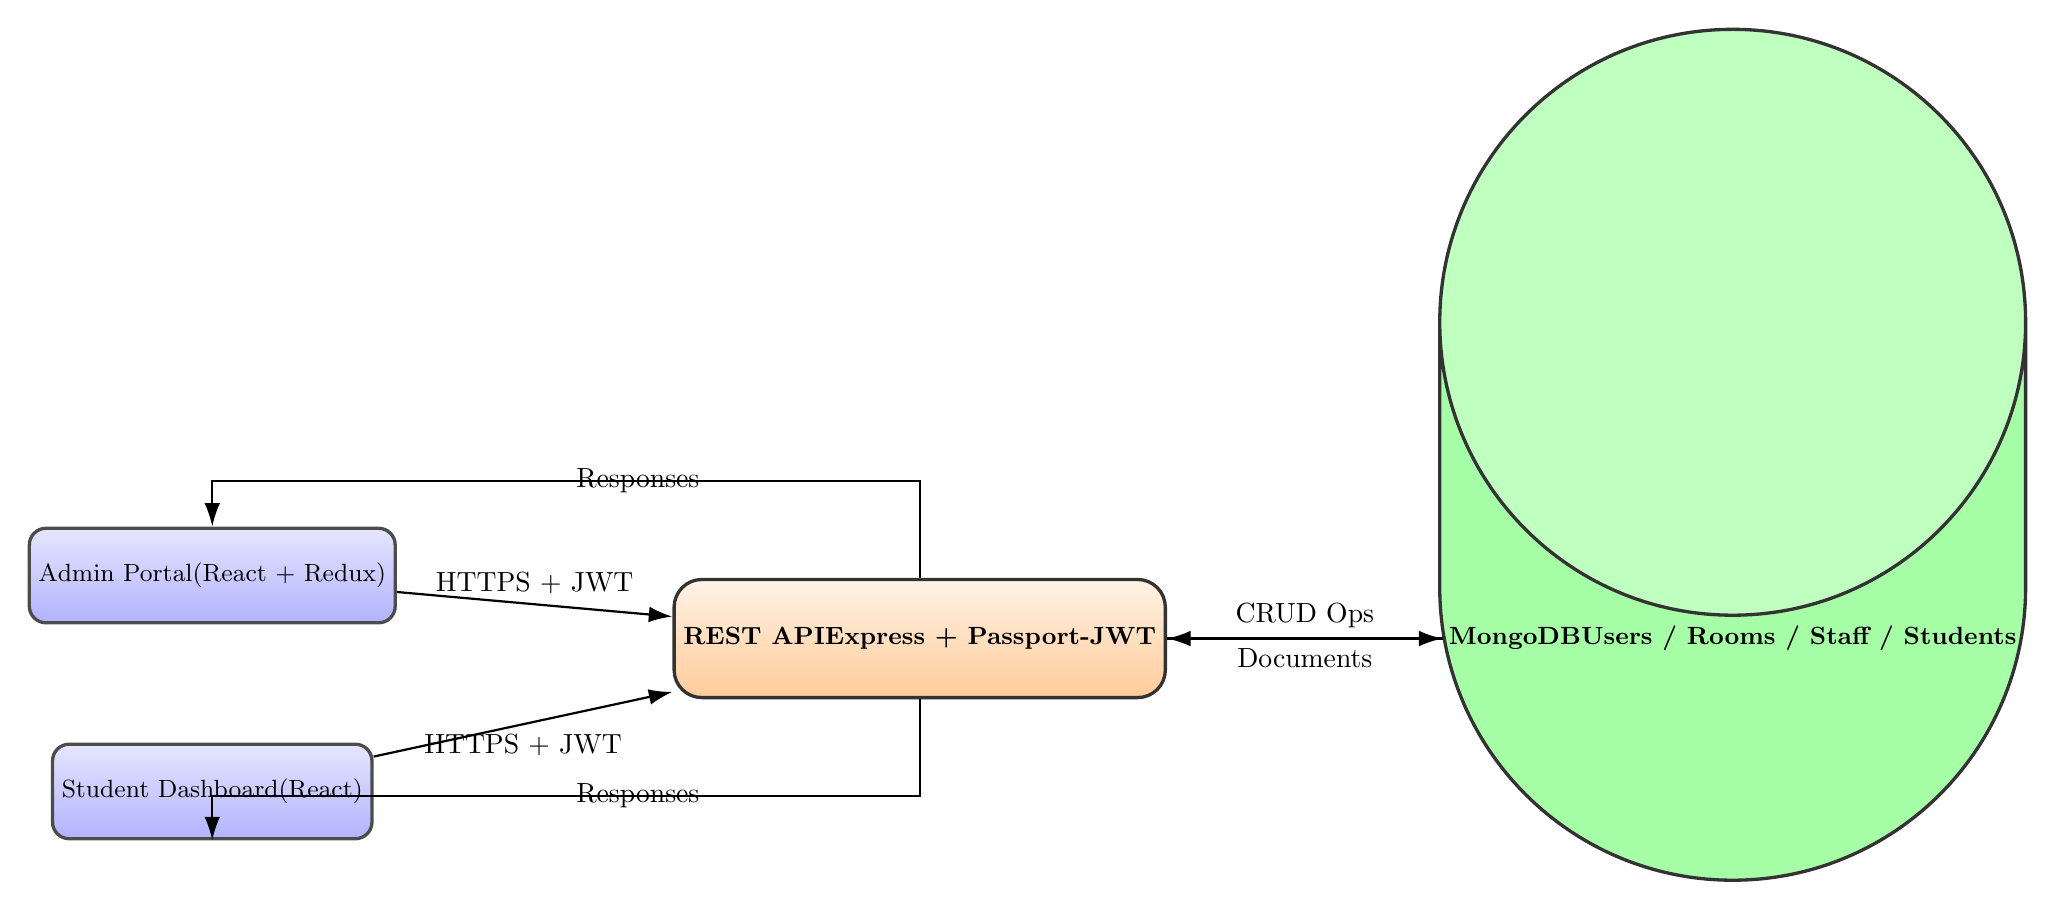
\begin{tikzpicture}[
      node distance=1.5cm and 3.5cm,
      client/.style={rectangle, rounded corners=6pt, draw=black!70, very thick,
                     minimum width=4cm, minimum height=1.2cm,
                     top color=blue!10, bottom color=blue!30, font=\small},
      service/.style={rectangle, rounded corners=10pt, draw=black!80, very thick,
                      minimum width=4.8cm, minimum height=1.5cm,
                      top color=orange!10, bottom color=orange!40, font=\small\bfseries},
      data/.style={cylinder, cylinder uses custom fill, cylinder body fill=green!35,
                   cylinder end fill=green!25, shape border rotate=90,
                   minimum height=2cm, minimum width=2.4cm, draw=black!80, very thick,
                   font=\small\bfseries},
      arrow/.style={-{Latex[length=3mm,width=2mm]}, thick}
    ]
    \node[client] (admin) {Admin Portal \\ (React + Redux)};
    \node[client, below=of admin] (student) {Student Dashboard \\ (React)};
    \node[service, right=of admin, yshift=-0.8cm] (api) {REST API \\ Express + Passport-JWT};
    \node[data, right=of api] (db) {MongoDB \\ Users / Rooms / Staff / Students};

    \draw[arrow] (admin) -- node[above]{HTTPS + JWT} (api);
    \draw[arrow] (student) -- node[below]{HTTPS + JWT} (api);
    \draw[arrow] (api) -- node[above]{CRUD Ops} (db);
    \draw[arrow] (db) -- node[below]{Documents} (api);
    \draw[arrow] (api) -- ++(0,2) -| node[pos=0.25,right]{Responses} (admin);
    \draw[arrow] (api) -- ++(0,-2) -| node[pos=0.25,right]{Responses} (student);
  \end{tikzpicture}
  \caption{High-level system architecture}
\end{figure}

\section{Acceptance Criteria}
\begin{itemize}
  \item Successful login/logout flows for admin and student roles.
  \item CRUD actions for students/rooms/staff restricted to admin tokens.
  \item Dashboards render current data and respond within acceptable time.
  \item Unit test suite executes (with mocked DB or isolated ports) covering user, student, and room APIs.
\end{itemize}

\end{document}

